\chapter{評価}
\label{chap:evaluation}

\ref{chap:video-production}章ての映像制作現場におけるIP伝送装置の要件に基づいて、ソフトウェア、ハードウェアそれぞれIP伝送装置の実装を行った。
本章ではアプローチが有効な手法であるか、それぞれの項目について評価する。

\section{概要}

\ref{chap:implementation}章と\ref{chap:implementation}章で実装したIP伝送装置を動作させる。
\ref{chap:video-production}章で要件としてあげた、トラフィックと遅延の2つの項目において計測手法をまとめ、計測結果とともに考察をまとめる。

\section{トラフィック}

本節では、実装したIP伝送装置が理想通りにパケットの送信を行っているかを確認するために、Linux PCを用いてトラフィックを計測した。

\subsection{計測手法}

ソフトウェア実装の場合はにおける受信PC、ハードウェア実装の場合はIP分配折り返しボードに接続されたデバッグ用のPCで、受信バイト数、受信パケット数、破棄パケット数を計測した。
ネットワークインターフェースの情報は/proc/net/devを監視した。rrdtoolを使い集計し、グラフとして出力した。

\subsection{計測結果}

ソフトウェア実装における計測結果を、図~\ref{fig:lo-bytes-graph}と図~\ref{fig:lo-packets-graph}に示す。

図~\ref{fig:lo-bytes-graph}で示した受信バイトのグラフでは、平均489MBpsとなっている。
ソフトウェア実装での映像データはYCbCr 4:2:2の色深度が16bitであるため、ピクセルあたり2bytesとなる。% また、フレームレートは30Pである。
理想的な1秒あたりの映像データのバイト数は、次のように求められる。

\[ 3840 \times 2160 \times 2 \times 30 = 497664000 \]

% ヘッダー60byte
% 489MBps

理想的な1秒あたりの受信バイト数を満たしていない。
この原因としては、送信PCがデータの送信に追いつかない場合に自動的にフレームをドロップさせる処理によるものだと考えられる。

ハードウェア実装における計測結果を、図~\ref{fig:enp2s0f1-bytes-graph}と図~\ref{fig:enp2s0f1-packets-graph}に示す。
図~\ref{fig:enp2s0f1-packets-graph}で示した受信パケットのグラフでは、パケットがドロップしている事が確認できる。
これは、カーネルのネットワーク処理が、FPGAのハードウェアによる出力の速度に追いつけなかったためだと考えられる。
ハードウェア実装での映像データはYCbCr 4:2:2の色深度が12bitとなる。ピクセルあたり2bytesとなる。
理想的な1秒あたりの映像データのバイト数は、次のように求められる。

\[ 3840 \times 2160 \times 2 \times 30 = 497664000 \]

カーネルが処理した1パケットあたりの平均バイト数$B_{avr}$は、受信したバイト数$B_{rcv}$、受信したパケット数$P_{rcv}$を用いて、次のように求められる。

\[ B_{avr} = \frac{B_{rcv}}{P_{rcv}} \]

本来PCが受信したであろうバイト数$B_{all}$は、1パケットあたりの平均バイト数$B_{avr}$、受信したパケット数$P_{rcv}$、破棄したパケット数$P_d$を用いて、次のように求められる。

\[ B_{all} = (P_{rcv} + P_d) \times B_{avr} \]

パケットには、ヘッダーとフッターが56bytes存在しているため、受信バイトのうち有効データ率$R_{vld}$は、1パケットあたりの平均バイト数$B_{avr}$を用いて、次のように求められる。

\[ R_{vld} = 1 - \frac{56}{B_{avr}} \]

このとき、1秒あたりの映像データのバイト数$B_{video}$は、次のように求められる。

\[ B_{video} = R_{vld} \times B_{avr} \]

図~\ref{fig:enp2s0f1-bytes-graph}と図~\ref{fig:enp2s0f1-packets-graph}から読み取った値から、次のように求められる。
\[ B_{avr} = \frac{694800066.36}{5437845.10} = 127.77 \]
\[ B_{all} = (5437845.10 + 1494269.10) \times 127.77 = 885716231 \]
\[ R_{vld} = 1 - \frac{56}{127.77} = 0.5617 \]
\[ B_{video} = 885716231 \times 0.5617 = 497506806 \]

$B_{video}$は、おおよそ理想的な1秒あたりの映像データのバイト数と一致している。

\begin{figure}[htbp]
  \begin{center}
    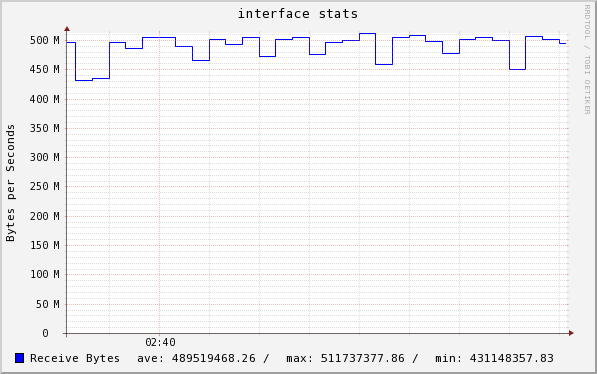
\includegraphics[bb=0 0 597 374,width=11.8cm]{img/lo-bytes-graph.png}
  \end{center}
  \caption{ソフトウェア実装における伝送中の受信バイトのグラフ}
  \label{fig:lo-bytes-graph}
\end{figure}

\begin{figure}[htbp]
  \begin{center}
    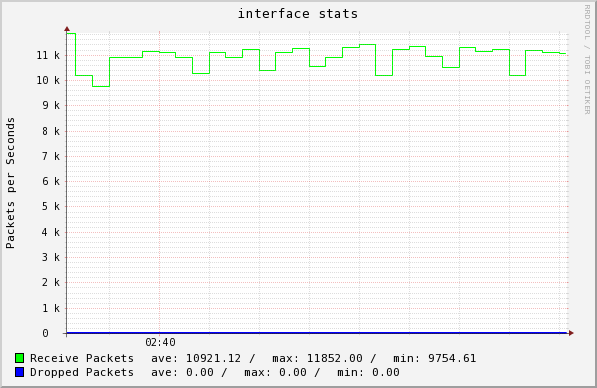
\includegraphics[bb=0 0 597 388,width=11.8cm]{img/lo-packets-graph.png}
  \end{center}
  \caption{ソフトウェア実装における伝送中の受信パケットのグラフ}
  \label{fig:lo-packets-graph}
\end{figure}

\begin{figure}[htbp]
  \begin{center}
    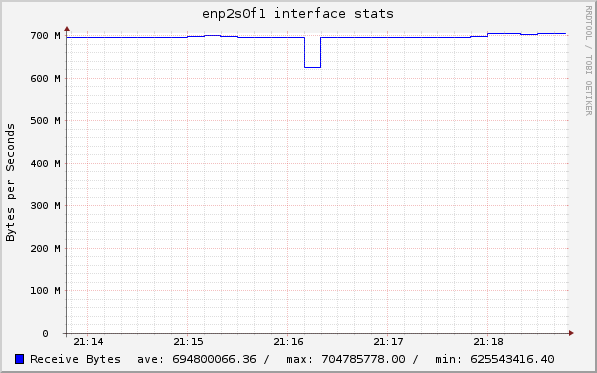
\includegraphics[bb=0 0 597 374,width=11.8cm]{img/enp2s0f1-bytes-graph.png}
  \end{center}
  \caption{ハードウェア実装における伝送中の受信バイトのグラフ}
  \label{fig:enp2s0f1-bytes-graph}
\end{figure}

\begin{figure}[htbp]
  \begin{center}
    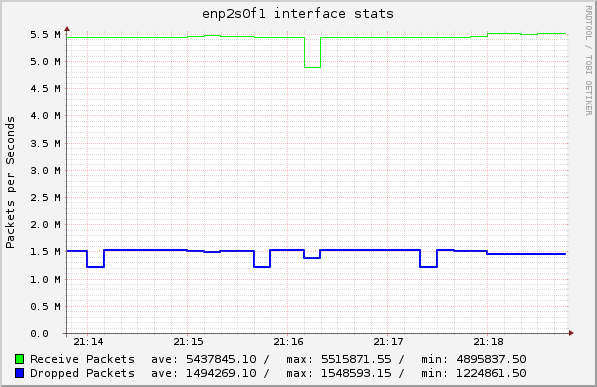
\includegraphics[bb=0 0 597 388,width=11.8cm]{img/enp2s0f1-packets-graph.png}
  \end{center}
  \caption{ハードウェア実装における伝送中の受信パケットのグラフ}
  \label{fig:enp2s0f1-packets-graph}
\end{figure}


\newpage
\section{遅延}

本節では、実装したIP伝送装置で映像制作現場において許容できる遅延の範囲内かを顕彰するために、遅延を計測する環境を用意し、発生する遅延を計測した。

\subsection{計測手法}

映像機器の遅延を計測するため、テスト信号生成、マルチビューワー生成、画面キャプチャーの機能を有する機器を用意した。
遅延を計測した機器の構成を図~\ref{fig:evaluate-diagram}に示す。

テスト信号生成では、フレーム単位のタイムコードが表示された同じソースの映像を2つの信号として出力する。
一方をスイッチャーへ入力し、もう一方を検査対象となる機器に入力し、その出力をスイッチャーへ入力する。
これにより、2つの信号の遅延は、検査対象となる機器で発生した遅延に抑えることができる。
スイッチャーに入力された2つの信号はマルチビューワーとして1つの画面に表示され、その画面をキャプチャーすることにより、ある瞬間の2つの信号を1つの画像で確認することができる。
このスイッチャーには、フレーム同期の機能があり、1フレームより短い期間でバッファリングされるため、計測できる粒度はフレーム単位となる。

\begin{figure}[htbp]
  \begin{center}
    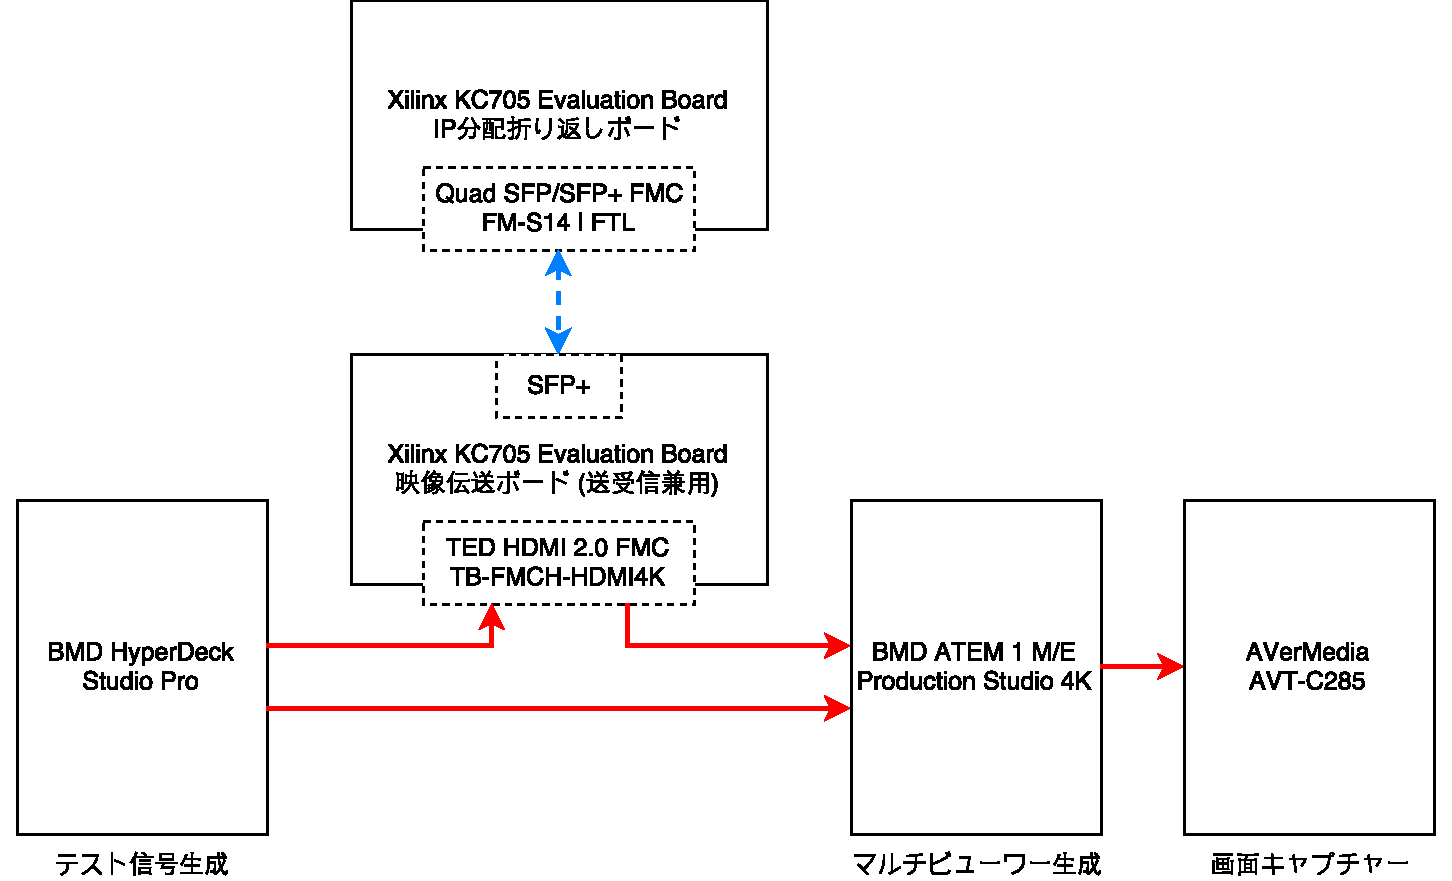
\includegraphics[bb=0 0 697 212,width=15cm]{img/evaluate-diagram.pdf}
  \end{center}
  \caption{遅延の計測手法}
  \label{fig:evaluate-diagram}
\end{figure}

キャプチャーした瞬間によっては、IP伝送装置のタイミングにより遅延のバラ付きが出る可能性があるため、5回計測を行う。
テスト信号はYCbCr 4:2:2の4K 30Pである。

\subsection{計測結果}

\begin{figure}[htbp]
  \begin{center}
    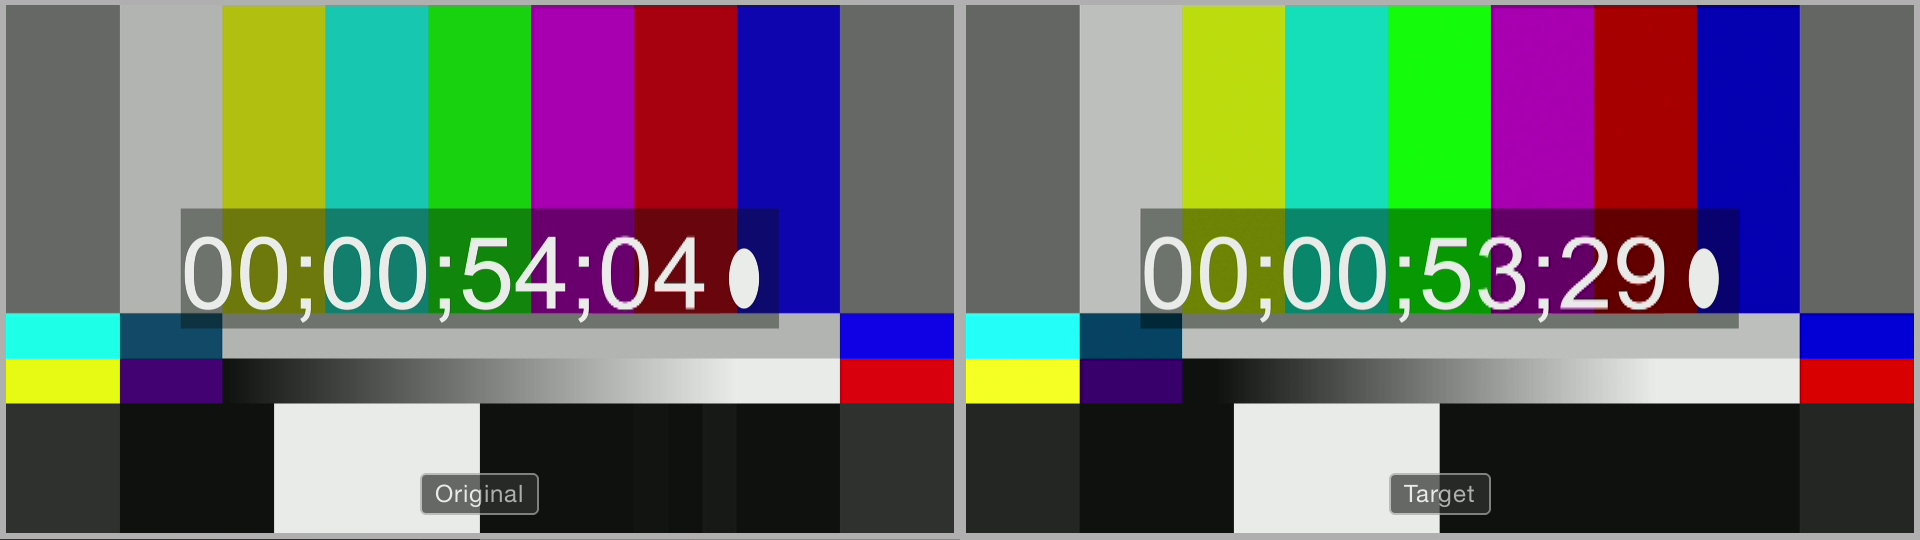
\includegraphics[bb=0 0 1920 540,width=14cm]{img/evaluate-delay-software-1.png}
  \end{center}
  \caption[ソフトウェア実装による1回目の遅延計測のキャプチャー画像]{\shortstack{左がオリジナルの信号、右が検査対象の信号\\ソフトウェア実装による1回目の遅延計測のキャプチャー画像}}
  \label{fig:evaluate-delay-software-1}
\end{figure}

\begin{figure}[htbp]
  \begin{center}
    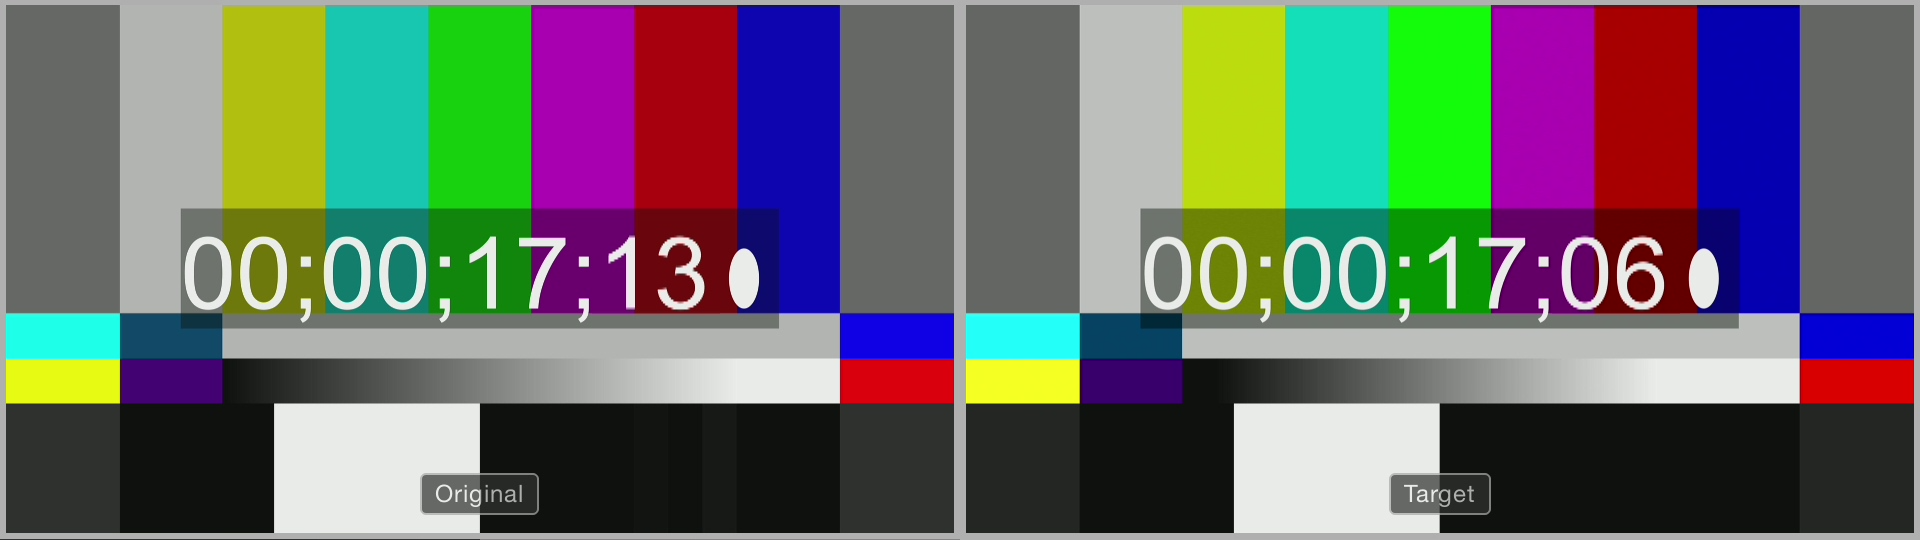
\includegraphics[bb=0 0 1920 540,width=14cm]{img/evaluate-delay-software-2.png}
  \end{center}
  \caption[ソフトウェア実装による4回目の遅延計測のキャプチャー画像]{\shortstack{左がオリジナルの信号、右が検査対象の信号\\ソフトウェア実装による4回目の遅延計測のキャプチャー画像}}
  \label{fig:evaluate-delay-software-2}
\end{figure}

\begin{figure}[htbp]
  \begin{center}
    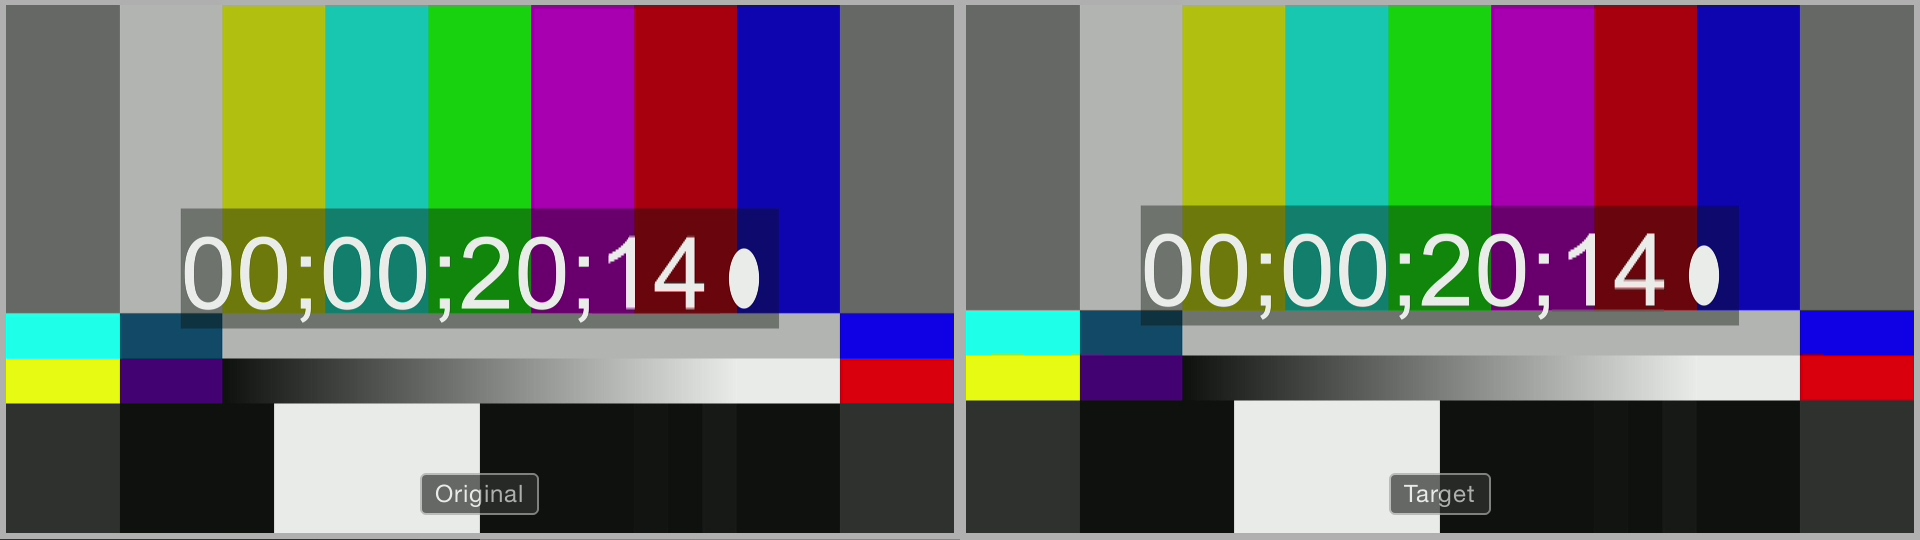
\includegraphics[bb=0 0 1920 540,width=14cm]{img/evaluate-delay-hardware.png}
  \end{center}
  \caption[ハードウェア実装による遅延計測のキャプチャー画像]{\shortstack{左がオリジナルの信号、右が検査対象の信号\\ハードウェア実装による遅延計測のキャプチャー画像}}
  \label{fig:evaluate-delay-hardware}
\end{figure}

% \section{YCbCr 4:2:0}
% あああ

ソフトウェア実装による遅延時間の計測の様子を図~\ref{fig:evaluate-delay-software-1}と図~\ref{fig:evaluate-delay-software-2}に示す。
また、計測結果を表~\ref{tb:evaluate-software-delay}に示す。
ハードウェアよりも遅延が多く、計測回数によってばらつきがあることが分かる。
遅延フレームの平均は6フレームとなり、30FPSでは199.99msとなる。
これは、\ref{chap:video-production}章で述べた、要件となる133.33msの遅延よりも多く、ソフトウェアによる実装では、映像制作現場に適さないことが分かる。

\begin{table}[htbp]
  \caption{ソフトウェア実装による30FPSにおける遅延時間の計測結果}
  \label{tb:evaluate-software-delay}
  \begin{center}
  \begin{tabular}{l|r}
    \hline
     計測回数 & 遅延フレーム \\\hline\hline
     1回目 & 6フレーム   \\\hline
     2回目 & 6フレーム   \\\hline
     3回目 & 3フレーム   \\\hline
     4回目 & 7フレーム   \\\hline
     5回目 & 9フレーム   \\\hline\hline
      平均 & 6フレーム   \\\hline
  \end{tabular}\end{center}
\end{table}

ハードウェア実装による遅延時間の計測を5回行ったが、遅延フレームはすべて0フレームであった。
計測環境の制限から遅延は1フレーム以内であるという結果になった。
要件となる遅延時間よりも短く、ハードウェアによる実装では、映像制作現場におけるIP伝送装置として優位であることが分かる。

% \section{実証実験}
% 本実装に実用性があることを顕彰するため、ORF2015とORF2016でそれぞれ実証実験を行った。
% 付録\ref{chap:orf2015}、付録\ref{chap:orf2016}

\section{考察}

ハードウェアによる実装では、YCbCr 4:2:0方式が使えるに加え、遅延も1フレーム以内であり、映像制作現場において優位に扱えることがわかった。
一方、ソフトウェアによる実装では、遅延が平均で6フレームとなり、映像制作現場における要件である133.33ms以内に抑えることができなかった。
